\documentclass[Rapport/Rapport_main.tex]{subfiles}
\begin{document}
\section{Indledning}
\subsection{Motivation og kontekst}
Mange mennesker har ikke egen bil af økonomiske eller praktiske årsager og er derfor nødsaget til at anvende offentlige transportmidler eller samkørsel. Der opstår dog ofte situationer, hvor det er fordelagtigt at have en bil til rådighed. Derfor har flere private aktører lanceret applikationer, hvor man som privatperson kan udleje sin bil, eller lease en andens bil i en periode. Et eksempel på et sådant firma er GoMore, der har udviklet en platform, som skal forsimple udlejningsprocessen og formidle kontakt mellem lejer og udlejer. Brugernes reviews indikerer imidlertid, at der er væsentlige problemer forbundet med brugen af platformen. \\\\Der skrives bl.a. på Trustpilot, at GoMore afkræver for høje gebyrer i forbindelse med udleje og forsikring, og at afgifterne stiger med tiden.\footnote{husk ref's} Mange vil derfor ikke længere anvende tjenesten af økonomiske årsager. Derudover klages der over en aflysningspolitik, som giver udlejer mulighed for at aflyse en handel kort før tid, til stor frustration for lejeren.\footnote{https://dk.trustpilot.com/reviews/5c5dbb0697afa10734cacfe6} Visse brugere nævner, at de ikke er trygge ved tjenesten på grund af manglende gennemsigtighed fra GoMore\footnote{https://dk.trustpilot.com/reviews/5c4b5d7b97afa10ac083141b}, mens andre giver udtryk for, at der mangler tillid mellem lejer og udlejer.\footnote{ref} \\\\Det fremgår, at mange af brugerne er utilfredse og leder efter alternativer. Der er således behov for et produkt, som simplificerer processen, og giver brugerne mulighed for at leje og udleje biler, uden at de bliver tynget af høje gebyrer og afgifter. Tjenesten skal udgøre en tryg ramme for udlejningsprocessen, så der opstår tillid mellem lejer og udlejer.

\subsection{Projektformulering}
Dette projektarbejde tager udgangspunkt i projektoplægget til 4. semester IKT på Aarhus Universitet\footnote{ref}. Der arbejdes derfor efter en iterativ udviklingsproces, hvor semesterets kurser integreres. Formålet er at implementere og teste et software udviklingsprojekt. Der anvendes objektorienteret analyse og design i udviklingen af en applikation, som har en grafisk brugergrænseflade og en database.\\\\Målet for dette projekt er at udvikle en funktionel prototype af en biludlejningsapplikation. Systemet skal give privatpersoner mulighed for at udleje og leje biler, mens udlejningsprocessen simplificeres mest muligt. Både lejere og udlejere skal kunne registrere sig som brugere gennem brugergrænsefladen, og systemet skal gemme informationer vedrørende brugere og biler. Det skal være nemt for lejer at søge efter biler og leje en ønsket bil, ud fra nogle kriterier. Det kunne f.eks. være en maksimumspris eller en maksimal afstand til bilen. Applikationen skal kunne tilgås på flere platforme, herunder Web, PC og Smartphone.

\subsection{Hvad er og kan vores system} 
Produktet som ønskes udviklet er en applikation kaldet CarnGo, der skal fungere både i en browser, på PC og på Smartphone. CarnGo skal løse nogle af de problemer, som er forbundet med etablerede biludlejningstjenester såsom GoMore. Applikationen skal give privatpersoner mulighed for at udleje biler i et tidsrum og til en pris, som de selv specificerer. Dermed får lejere mulighed for at vælge mellem tilgængelige biler og leje den bil, som opfylder netop deres behov. \\\\For at CarnGo bliver en brugervenlig applikation, som kan konkurrere med lignende tjenester, er der visse funktionaliteter, som den nødvendigvis må indeholde. Det skal være muligt at oprette en brugerprofil som henholdsvis lejer eller udlejer, alt efter om man ønsker at lease en andens bil, eller stille sin egen bil til rådighed. Som udlejer skal man kunne oprette en bilprofil, der indeholder relevante informationer vedrørende bilen. Efter oprettelsen kan man logge ind på sin profil på applikationen og redigere/slette sin brugerprofil eller bilprofiler.
\\\\Lejere skal have mulighed for at søge mellem de oprettede bilprofiler, til de finder en bil, som opfylder deres krav. Når der skal indgås en aftale om leje af en bil, er der behov for et besked- eller notifikationssystem mellem lejer og udlejer. Det skal således være muligt for lejer at anmode om leje af bil, og udlejer skal have mulighed for at reagere på anmodningen med en godkendelse eller afvisning.\\Funktionaliteten skal integreres med en brugergrænseflade, som er lettilgængelig og intuitiv at anvende, for at sikre den bedst mulige brugeroplevelse.

\subsection{Skitse af system}
Ud fra ovenstående beskrivelse er der udarbejdet en skitse, som viser, hvordan der interageres med applikationen CarnGo. Denne er vist i figur \ref{fig:CarnGo_skitse}.

\begin{figure}[H]
    \centering
    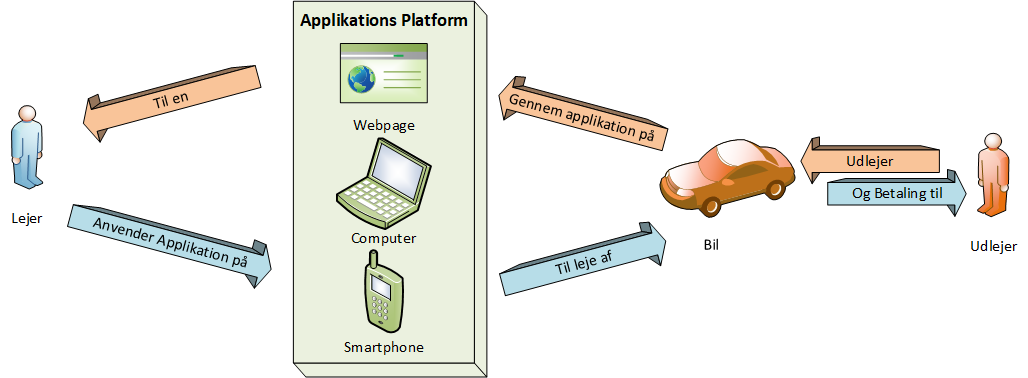
\includegraphics[width=\textwidth]{Projektformulering/graphic/SystemSkitsePRJ4.png}
    \caption{Skitse af CarnGo}
    \label{fig:CarnGo_skitse}
\end{figure}
\end{document}